% Session 4: Advanced Claude Code --- Skills, MCPs, Subagents
% Beamer Presentation --- Claude Code for Academic Researchers
\documentclass[aspectratio=169, 11pt]{beamer}

% ── Theme and Colors ──────────────────────────────────────────────
\usetheme{Madrid}
\usecolortheme{default}

\definecolor{anthropic}{RGB}{50, 50, 80}
\definecolor{accent}{RGB}{180, 90, 40}
\definecolor{lightgray}{RGB}{245, 245, 245}

\setbeamercolor{structure}{fg=anthropic}
\setbeamercolor{frametitle}{bg=anthropic, fg=white}
\setbeamercolor{title}{bg=anthropic, fg=white}
\setbeamercolor{block title}{bg=anthropic, fg=white}
\setbeamercolor{block body}{bg=lightgray}
\setbeamercolor{alerted text}{fg=accent}

\setbeamerfont{title}{size=\Large, series=\bfseries}
\setbeamerfont{frametitle}{size=\large, series=\bfseries}

% ── Packages ──────────────────────────────────────────────────────
\usepackage{graphicx}
\usepackage{booktabs}
\usepackage{listings}
\usepackage{fontenc}
\usepackage{hyperref}
\usepackage{tikz}
\usetikzlibrary{positioning}

\lstset{
  basicstyle=\ttfamily\small,
  backgroundcolor=\color{lightgray},
  frame=single,
  framerule=0pt,
  breaklines=true,
  columns=fullflexible,
  literate={_}{\_}1,
}

% ── Metadata ──────────────────────────────────────────────────────
\title{Session 4: Advanced Claude Code}
\subtitle{Skills, MCPs, and Subagents}
\author{Brady Allardice}
\date{}
\institute{UPF \& IBEI}

% ══════════════════════════════════════════════════════════════════
\begin{document}

% ── Title ─────────────────────────────────────────────────────────
\begin{frame}[plain]
  \titlepage
\end{frame}

% ══════════════════════════════════════════════════════════════════
%  WHERE WE ARE
% ══════════════════════════════════════════════════════════════════

\begin{frame}{Where We Are}
  \textbf{Session 1:} What Claude Code can do. How it works. CLAUDE.md and plan mode.

  \vspace{0.4em}
  \textbf{Session 2:} The core workflow. Data cleaning, estimation, robustness, \LaTeX{} tables.

  \vspace{0.4em}
  \textbf{Session 3:} Git and \LaTeX{} in VS Code. Your paper joins the project.

  \vspace{0.4em}
  \textbf{Session 4:} The layer above the core workflow --- infrastructure.

  \vspace{1em}
  Today you will:
  \begin{enumerate}
    \item Migrate to a cleaner repo workflow (a structural fix, not an agent fix)
    \item Build a framework for deciding when a \textbf{skill} earns its keep
    \item Connect two \textbf{MCPs} (Zotero, GitHub) and use them in practice
    \item Learn when to reach for a \textbf{subagent} --- and when not to
  \end{enumerate}

  \vspace{0.5em}
  \alert{Today is about knowing which tool does real work and which is just novelty.}
\end{frame}

\begin{frame}{Check-In}
  \textbf{Since Session 3:}

  \vspace{0.6em}
  \begin{itemize}
    \item Did the git cycle (commit $\rightarrow$ instruct $\rightarrow$ diff $\rightarrow$ decide) stick?
    \item Did anyone bring their paper into VS Code? How did it feel?
    \item Any tool fight back at you --- compilation errors, merge conflicts, something else?
  \end{itemize}

  \vspace{0.8em}
  Hold onto the merge-conflict stories. We start there.
\end{frame}

% ══════════════════════════════════════════════════════════════════
%  PART 1: GIT RESTRUCTURING + META-LESSON
% ══════════════════════════════════════════════════════════════════

\begin{frame}{Part 1: A Workflow Fix Before We Start}
  \centering
  \vspace{2em}
  {\Large Agents solve symptoms well.\\[0.3em]
  They do not notice when a problem shouldn't exist.}

  \vspace{2em}
  Fifteen minutes. One migration. The meta-lesson for the rest of the session.
\end{frame}

\begin{frame}{The Problem We Had}
  \textbf{Every session so far, someone has hit a merge conflict.}

  \vspace{0.6em}
  What we did about it:
  \begin{itemize}
    \item Deleted the local repo and recloned
    \item Asked Claude Code to resolve the conflict markers
    \item Copied work to the Desktop, wiped the directory, copied back
  \end{itemize}

  \vspace{0.8em}
  \textbf{That worked.} Everyone got unstuck. But it was a symptom fix.

  \vspace{0.8em}
  \begin{alertblock}{The Root Cause}
    You were editing files \emph{inside} the shared course repository. Every time I pushed new material, git had to reconcile your changes with mine. Conflicts were guaranteed by the structure, not by accident.
  \end{alertblock}
\end{frame}

\begin{frame}[fragile]{The Structural Fix}
  \textbf{New layout on my side:} each session is a self-contained folder.

  \vspace{0.3em}
  \begin{lstlisting}[basicstyle=\ttfamily\footnotesize]
AIAgentsCourse/
  session_1/
  session_2/
  session_3/
  session_4/     <- today's materials live here
  ...
  \end{lstlisting}

  \vspace{0.5em}
  \textbf{New workflow on your side:} copy the session folder out of the repo into your own workspace. Work there. The shared repo stays read-only for you.

  \vspace{0.6em}
  \begin{block}{What this changes}
    I can push new material anytime without breaking anything in your workspace. You can edit, break, delete, and redo without worrying about the shared state. No more conflicts.
  \end{block}
\end{frame}

\begin{frame}[fragile]{The Three-Step Ritual}
  \textbf{Do this at the start of every session from now on:}

  \vspace{0.5em}
  \begin{lstlisting}[basicstyle=\ttfamily\footnotesize]
# 1. Pull the latest course repo
cd ~/AIAgentsCourse && git pull

# 2. Copy today's session folder into your workspace
cp -r session_4/ ~/my_workspace/session_4/

# 3. Open your copy in VS Code and work there
cd ~/my_workspace/session_4 && code .
  \end{lstlisting}

  \vspace{0.5em}
  \textbf{We do it together now, live.} Five minutes. Everyone ends up in the same clean state before we move on.

  \vspace{0.5em}
  {\small If you had in-progress work inside the course repo, copy it into \texttt{\textasciitilde/my\_workspace/} too. I will help you sort out what to keep.}
\end{frame}

\begin{frame}{The Meta-Lesson}
  \textbf{Agents solve symptoms well. They do not notice when a problem shouldn't exist.}

  \vspace{0.8em}
  Claude Code could have resolved merge conflicts forever. It was good at it. What it would not have done is stop and say: \emph{``Why are you editing the shared repo in the first place?''}

  \vspace{0.8em}
  \textbf{Your job, not the agent's:} when a symptom keeps recurring, ask whether the structure is wrong.

  \vspace{0.8em}
  \begin{block}{A question to carry with you}
    When you catch yourself reaching for Claude Code to patch the same thing a third time, pause. Is there a structural fix you're missing?
  \end{block}

  \vspace{0.5em}
  This lesson lands again when we talk about skills (are you using it, or did you just build it?) and MCPs (does this earn a permanent connection, or is it just novelty?).
\end{frame}

% ══════════════════════════════════════════════════════════════════
%  PART 2: SKILLS DEEP-DIVE (CENTERPIECE)
% ══════════════════════════════════════════════════════════════════

\begin{frame}{Part 2: Skills}
  \centering
  \vspace{2em}
  {\Large What they are.\\[0.3em]
  When they earn their keep.\\[0.3em]
  When they do not.}

  \vspace{2em}
  The centerpiece of today.
\end{frame}

% ---- 2a: What skills are + taxonomy ------------------------------

\begin{frame}{Skills, Defined}
  \textbf{A skill is a reusable instruction bundle that Claude Code loads when relevant.}

  \vspace{0.6em}
  \begin{itemize}
    \item Invoked by name: \texttt{/skill-name}
    \item Or auto-triggered when the description matches what you are doing
    \item Lives in \texttt{.claude/skills/<name>/SKILL.md}
    \item Can include helper scripts alongside the instruction file
  \end{itemize}

  \vspace{0.8em}
  \textbf{Think of it as:}
  \begin{itemize}
    \item CLAUDE.md sets \emph{project-wide} conventions. Always on.
    \item A skill encodes a \emph{specific task}. Loads when you need it.
  \end{itemize}

  \vspace{0.5em}
  \begin{block}{The one-sentence definition}
    A skill is a named, reusable prompt with enough structure that it's worth loading on demand.
  \end{block}
\end{frame}

\begin{frame}[fragile]{Anatomy of a Skill}
  A \texttt{SKILL.md} looks like this:

  \vspace{0.3em}
  \begin{lstlisting}[basicstyle=\ttfamily\footnotesize]
---
name: spec-validator
description: Validate data, variables, and transformations
  BEFORE estimation. Use when the user is about to run a
  regression, has loaded data, or mentions specification.
---

# Instructions

Before any estimation, verify:
1. Variable types match the spec ...
2. Missing data handling is explicit ...
3. Sample sizes are reported ...
[... full instructions ...]
  \end{lstlisting}

  \vspace{0.2em}
  \textbf{The description is what earns the skill its load.} Claude Code reads it on every turn and decides whether this skill is relevant.

  \vspace{0.2em}
  \alert{Specific enough to be useful. Narrow enough not to misfire.}
\end{frame}

\begin{frame}{Skill vs. Prompt vs. CLAUDE.md}
  \textbf{The key question:} when is something worth being a skill?

  \vspace{0.6em}
  \begin{itemize}
    \item \textbf{Just prompt} --- one-off, simple, low stakes.\\
    {\small Example: ``Rename this variable from \texttt{x} to \texttt{income}.''}

    \vspace{0.3em}
    \item \textbf{CLAUDE.md entry} --- project-wide convention, always on.\\
    {\small Example: ``Use pandas for data manipulation.''}

    \vspace{0.3em}
    \item \textbf{Skill} --- task-specific, recurring, carries non-trivial structure or knowledge.\\
    {\small Example: ``Before estimation, run these 12 validation checks.''}
  \end{itemize}

  \vspace{0.8em}
  \begin{alertblock}{The test question}
    Would a fresh prompt do this just as well? If yes, it's not a skill --- it's a habit you can write down. If no, ask: what is the skill actually carrying?
  \end{alertblock}
\end{frame}

\begin{frame}{A Taxonomy for Evaluating Skills}
  \textbf{A skill earns its keep when it is doing one of these things:}

  \vspace{0.6em}
  \begin{enumerate}
    \item \textbf{Domain knowledge} --- encodes facts the model would miss otherwise.\\
    {\small Discipline-specific conventions, clustering rules, staggered-DiD pitfalls.}

    \vspace{0.3em}
    \item \textbf{Workflow structure} --- enforces a multi-step procedure you'd otherwise skip steps of.\\
    {\small A 12-step validation protocol; a structured robustness battery.}

    \vspace{0.3em}
    \item \textbf{Critique / persona} --- applies a specific lens the model wouldn't spontaneously adopt.\\
    {\small ``Read this as a skeptical referee.'' ``Audit this for replication errors.''}

    \vspace{0.3em}
    \item \textbf{Output format} --- produces artifacts with a rigid shape.\\
    {\small Codebook entries; decision-log lines; LaTeX tables in your house style.}
  \end{enumerate}

  \vspace{0.5em}
  \alert{If a skill doesn't fit one of these four boxes, it's probably a habit pretending to be infrastructure.}
\end{frame}

\begin{frame}{The Test, Concretely}
  \textbf{For any candidate skill, ask three questions:}

  \vspace{0.8em}
  \begin{enumerate}
    \item \textbf{Would a fresh prompt produce the same output?}\\
    {\small If yes $\rightarrow$ not a skill.}

    \vspace{0.4em}
    \item \textbf{Which taxonomy category is it in?}\\
    {\small Domain knowledge / workflow / critique / format. If you can't name one, be suspicious.}

    \vspace{0.4em}
    \item \textbf{Will you actually invoke it?}\\
    {\small Skills you built and never use are dead weight. They clutter the description-matching space and make other skills worse.}
  \end{enumerate}

  \vspace{1em}
  \begin{block}{The honest version}
    Most people build more skills than they need. The discipline isn't in building them --- it's in culling them.
  \end{block}
\end{frame}

% ---- 2b: Critique demo (pedagogical heart) ----------------------

\begin{frame}{Demo: Critiquing My Own Skills}
  \textbf{I'm going to walk through my actual skill list.}

  \vspace{0.6em}
  \begin{itemize}
    \item Some clearly earn their keep --- I will say why.
    \item Some are marginal --- I will think out loud and let you watch me arrive at an honest answer.
    \item No skill gets a pass just because I built it.
  \end{itemize}

  \vspace{0.8em}
  \alert{This is the exercise I want you to be able to do for your own skills later.}

  \vspace{0.6em}
  \begin{block}{The stance}
    You will build skills. Some will be great. Some will be ceremony. The difference between a useful toolkit and a bloated one is whether you're willing to kill your own creations.
  \end{block}
\end{frame}

\begin{frame}[fragile]{My Current Skill List}
  From \texttt{\textasciitilde/.claude/skills/}:

  \vspace{0.3em}
  \begin{lstlisting}[basicstyle=\ttfamily\footnotesize]
spec-validator/       Validate data + specs before estimation
robustness-checks/    Structured robustness battery (panel,
                      2SLS, DiD, RDD)
research-docs/        Auto-maintain README + codebook +
                      decision log
auto-commit/          Install the auto-commit hook
  \end{lstlisting}

  \vspace{0.3em}
  \textbf{Plus a few global ones} (I'll mention but not dissect every one).

  \vspace{0.3em}
  We'll look at two in detail: one that clearly earns its keep, and one I'm less sure about.
\end{frame}

\begin{frame}{Earns Its Keep: \texttt{spec-validator}}
  \textbf{What it does:} before any regression, walks through variable types, value ranges, missingness patterns, merge diagnostics, clustering assumptions, scale mismatches.

  \vspace{0.6em}
  \textbf{Why it's a skill and not a prompt:}
  \begin{itemize}
    \item \textbf{Domain knowledge} --- encodes the dozen silent-error patterns that actually invalidate estimation (NaN coercion, wrong join keys, sample drops, improper clustering).
    \item \textbf{Workflow structure} --- a 12-step protocol I would skip half of if I prompted ad hoc.
  \end{itemize}

  \vspace{0.5em}
  \textbf{The fresh-prompt counterfactual:}
  \begin{itemize}
    \item ``Check my data before I run this regression'' misses most of what matters
    \item A fresh prompt catches maybe 3 of the 12 checks
  \end{itemize}

  \vspace{0.5em}
  \begin{block}{Verdict}
    Earns its keep. Two taxonomy categories. Clear value-added over a prompt.
  \end{block}
\end{frame}

\begin{frame}{Marginal Case: \texttt{research-docs}}
  \textbf{What it claims:} auto-maintain README + codebook + decision log as I work.

  \vspace{0.4em}
  \textbf{Walking through the test:}
  \begin{itemize}
    \item \emph{Fresh-prompt counterfactual:} could I just say ``log this in the codebook''? Mostly yes.
    \item \emph{Domain knowledge?} A little --- knows what belongs in a codebook vs.\ a README.
    \item \emph{Workflow structure?} Some --- the three files stay in sync. But that's format, not structure.
    \item \emph{Will I invoke it?} Honestly... sometimes. Often I just write a note.
  \end{itemize}

  \vspace{0.3em}
  \textbf{Thinking out loud:} probably a \emph{format} skill pretending to be a workflow one. Might earn its keep if I used it religiously. I don't.

  \vspace{0.3em}
  \begin{alertblock}{Honest verdict}
    Leaning: demote to a CLAUDE.md paragraph and a habit. I'd rather have three skills I use than ten I built.
  \end{alertblock}
\end{frame}

% ---- 2c: Hands-on ------------------------------------------------

\begin{frame}{Exercise 1: Evaluate Three Skills (8 min)}
  \textbf{Pairs. I'll put three skill descriptions on the screen.} For each, decide together:

  \vspace{0.6em}
  \begin{itemize}
    \item \textbf{Keep} --- it clearly fits the taxonomy and they would use it
    \item \textbf{Kill} --- a fresh prompt would do the same work
    \item \textbf{Demote} --- it's a CLAUDE.md line or a habit, not a skill
  \end{itemize}

  \vspace{0.8em}
  \textbf{For each one, name:}
  \begin{enumerate}
    \item Your verdict
    \item Which taxonomy category (if keep) or why not (if kill/demote)
  \end{enumerate}

  \vspace{0.8em}
  We'll share two or three answers as a group.

  \vspace{0.5em}
  \alert{Disagreement is the point. If everyone agrees, I picked the wrong examples.}
\end{frame}

\begin{frame}{Exercise 2: Sketch a Skill of Your Own (10 min)}
  \textbf{Individually, write a four-line spec for one skill you'd actually build for your own research.}

  \vspace{0.6em}
  \begin{enumerate}
    \item \textbf{Name}
    \item \textbf{One-sentence description}
    \item \textbf{Taxonomy category:} domain knowledge / workflow / critique / format
    \item \textbf{Why a fresh prompt wouldn't do it just as well}
  \end{enumerate}

  \vspace{0.8em}
  A few will share. No coding, no installation. The deliverable is the reasoning.

  \vspace{0.6em}
  \begin{block}{The bar}
    If you can justify it under the test question --- ``would a fresh prompt do this just as well?'' --- you have a skill. If you can't, you have a habit. Both are fine. They just live in different places.
  \end{block}
\end{frame}

\begin{frame}{Skills: What to Take Away}
  \textbf{You will leave this session with:}

  \vspace{0.6em}
  \begin{itemize}
    \item A vocabulary: domain knowledge / workflow / critique / format
    \item A test question: \emph{would a fresh prompt do this just as well?}
    \item An honest example of a marginal case, from my own toolkit
    \item One sketch of a skill you could build
  \end{itemize}

  \vspace{1em}
  \begin{alertblock}{What I did not give you}
    A step-by-step install guide. Building a working skill is about 15 minutes with the docs once you know you want one. Knowing whether you want one is the hard part --- and that's what today was about.
  \end{alertblock}

  \vspace{0.4em}
  {\small Pointer to the docs: \url{https://docs.claude.com/en/docs/claude-code/skills}}
\end{frame}

% ══════════════════════════════════════════════════════════════════
%  PART 3: MCPS
% ══════════════════════════════════════════════════════════════════

\begin{frame}{Part 3: MCPs}
  \centering
  \vspace{2em}
  {\Large Connecting Claude Code\\[0.3em]
  to systems outside your project.}

  \vspace{2em}
  Forty-five minutes. Two MCPs. One pair exercise.
\end{frame}

% ---- 3a: Framing -------------------------------------------------

\begin{frame}{What an MCP Is}
  \textbf{MCP = Model Context Protocol.} An open standard for plugging external tools into Claude Code.

  \vspace{0.6em}
  \begin{itemize}
    \item Each MCP is a separate server.
    \item Claude Code speaks to it over a standard protocol.
    \item The server exposes \emph{tools} (like \texttt{zotero\_search}) that Claude Code can call.
  \end{itemize}

  \vspace{0.8em}
  \textbf{Without MCPs:} Claude Code reads and writes files in your project. That's it.\\[0.2em]
  \textbf{With MCPs:} it can query your Zotero library, open a GitHub PR, read a database, post to Slack --- anything someone has built a server for.

  \vspace{0.8em}
  \begin{block}{The framing}
    MCPs turn Claude Code from a tool that operates on your \emph{files} into a tool that operates on your \emph{workflow}.
  \end{block}
\end{frame}

\begin{frame}{The Two-Reason Rule}
  \textbf{Build or adopt an MCP for exactly one of two reasons:}

  \vspace{0.6em}
  \begin{enumerate}
    \item \textbf{Extend capability.} Let Claude Code do something it couldn't do at all.\\
    {\small Example: open a GitHub pull request. Query your Zotero library. Run a SQL query against your database.}

    \vspace{0.4em}
    \item \textbf{Reduce friction at a boundary.} Let it do something you \emph{could} already do, but where context-switching between tools kills the flow.\\
    {\small Example: inserting citations while drafting. You could look them up in Zotero and paste. But stopping to do that breaks writing flow.}
  \end{enumerate}

  \vspace{0.8em}
  \alert{Today I'm showing two specific MCPs I think are worth adopting. There are dozens more. The \emph{framework} is what transfers; the two cases are how you learn it.}

  \vspace{0.4em}
  Callback to the meta-lesson: MCPs are easy to accumulate. Ask what each one earns.
\end{frame}

% ---- 3b: Zotero --------------------------------------------------

\begin{frame}{The Friction Case: Zotero}
  \textbf{Drafting with citations normally looks like:}

  \vspace{0.3em}
  \begin{enumerate}
    \item Write a sentence that needs a citation
    \item Stop. Open Zotero. Search. Find the paper. Copy the cite key.
    \item Come back to the editor. Paste. Context-switch back into drafting.
    \item Repeat ten times per paragraph.
  \end{enumerate}

  \vspace{0.5em}
  \textbf{With the Zotero MCP:} ``Find me the Smith 2019 paper on voter ID, add it to refs.bib, and cite it here.'' Claude Code does the search, the BibTeX export, the \texttt{\textbackslash cite\{\}} insertion --- without you leaving the \texttt{.tex} file.

  \vspace{0.5em}
  \begin{block}{Why it earns its keep}
    \textbf{Reduce friction at a boundary.} You could already do all of this manually. The MCP just removes the tool-switch.
  \end{block}
\end{frame}

\begin{frame}[fragile]{Zotero MCP: Live Demo}
  \textbf{A single prompt:}

  \vspace{0.3em}
  \begin{lstlisting}[basicstyle=\ttfamily\footnotesize]
Find three recent papers on voter ID laws from my
Zotero library, add them to refs.bib, and draft one
sentence citing each in methods.tex.
  \end{lstlisting}

  \vspace{0.4em}
  \textbf{What you'll see in the tool-call log:}
  \begin{enumerate}
    \item \texttt{zotero\_semantic\_search("voter ID laws")} --- finds candidates
    \item \texttt{zotero\_get\_item\_metadata(...)} --- pulls BibTeX fields for each
    \item \texttt{Write refs.bib} --- creates or appends to the bibliography
    \item \texttt{Edit methods.tex} --- inserts three sentences with \texttt{\textbackslash cite\{...\}}
  \end{enumerate}

  \vspace{0.5em}
  \alert{Watch the tool calls, not just the output. Seeing which tools fire tells you what the MCP actually does.}
\end{frame}

\begin{frame}{Where Would This Reduce Friction for You?}
  \textbf{One minute, with the person next to you:}

  \vspace{0.8em}
  \begin{itemize}
    \item Where in your own drafting workflow do you break flow to check Zotero?
    \item Is it frequent enough that removing the context-switch would actually matter?
    \item Or is it rare enough that the setup cost isn't worth it?
  \end{itemize}

  \vspace{1em}
  \begin{alertblock}{Installation is homework, not class time}
    Installing the Zotero MCP is fifteen minutes of fiddling with API keys and configuration files. I am not making you do it in class. Setup guide is in the Session 5 prework.
  \end{alertblock}
\end{frame}

% ---- 3c: GitHub + pair exercise ----------------------------------

\begin{frame}{The Capability Case: GitHub}
  \textbf{GitHub MCP lets Claude Code do things you couldn't do by just editing files:}

  \vspace{0.6em}
  \begin{itemize}
    \item Open a pull request from a branch you've been working on
    \item Leave review comments on a coauthor's PR
    \item Create issues to track tasks you don't want to lose
    \item Push files to a remote repository
  \end{itemize}

  \vspace{0.8em}
  \textbf{Why now?} This morning's Git restructuring put you in a clean state. You are working in your own workspace. You understand the three states: local copy, pushed branch, shared main. The GitHub MCP is what closes the collaboration loop.

  \vspace{0.5em}
  \begin{block}{Why it earns its keep}
    \textbf{Extend capability.} ``Open a PR'' isn't something Claude Code can do without this. It's a genuine new capability, not a friction fix.
  \end{block}
\end{frame}

\begin{frame}{The Mental Model}
  \centering
  \vspace{0.3em}
  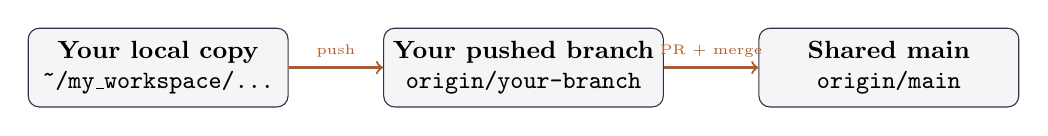
\begin{tikzpicture}[
    node distance=0.8cm and 1.2cm,
    box/.style={draw=anthropic, fill=lightgray, rounded corners, minimum width=3.3cm, minimum height=1cm, align=center, font=\small},
    arr/.style={->, thick, color=accent}
  ]
    \node[box] (local) {\textbf{Your local copy}\\ \texttt{\textasciitilde/my\_workspace/...}};
    \node[box, right=of local] (branch) {\textbf{Your pushed branch}\\ \texttt{origin/your-branch}};
    \node[box, right=of branch] (main) {\textbf{Shared main}\\ \texttt{origin/main}};

    \draw[arr] (local) -- node[above, font=\tiny] {push} (branch);
    \draw[arr] (branch) -- node[above, font=\tiny] {PR + merge} (main);
  \end{tikzpicture}

  \vspace{1em}
  \textbf{Branches + PRs are the collaboration mechanism.} The GitHub MCP is a \emph{helper} on top --- not a substitute.

  \vspace{0.5em}
  \begin{alertblock}{The discipline}
    Use \texttt{git} directly. Use the MCP when you're stuck or when the MCP genuinely saves steps. When things break, you need to understand what's actually happening --- and the MCP abstracts that away.
  \end{alertblock}
\end{frame}

\begin{frame}{Exercise Setup: Collaboration Pairs (5 min)}
  \textbf{Find a partner.} You will work as a pair for the next 25 minutes.

  \vspace{0.6em}
  \textbf{Each pair gets:} a link to a small template repo with 2--3 editable files and a README explaining the exercise.

  \vspace{0.6em}
  \textbf{The arc:}
  \begin{enumerate}
    \item Fork the template (each of you --- separate forks)
    \item Each makes a change on your own branch
    \item Open a PR on your partner's fork
    \item Partner reviews and merges
  \end{enumerate}

  \vspace{0.8em}
  \alert{Use Claude Code + the GitHub MCP to do the PR opening and reviewing. Use \texttt{git} directly for the commits and branches.}
\end{frame}

\begin{frame}{Exercise: The PR Loop (20 min)}
  \textbf{Pair workflow:}

  \vspace{0.3em}
  \begin{enumerate}
    \item \textbf{Fork} the template repo I shared in chat
    \item \textbf{Clone} your fork to \texttt{\textasciitilde/my\_workspace/}
    \item \textbf{Branch:} \texttt{git checkout -b my-change}
    \item \textbf{Edit} one of the files (different files for you and your partner)
    \item \textbf{Commit + push} the branch
    \item \textbf{Ask Claude Code} to open a PR using the GitHub MCP:\\[0.2em]
    \quad \emph{``Open a PR from my-change to main on my fork with title X and body Y.''}
    \item \textbf{Partner reviews} the PR (also via Claude Code + GitHub MCP) and merges it
  \end{enumerate}

  \vspace{0.4em}
  \textbf{Extension, if you finish early:} each edit the \emph{same} file, hit a conflict, resolve it together.

  \vspace{0.3em}
  {\small I will circulate. Flag me when you're stuck --- don't silently spin.}
\end{frame}

\begin{frame}{What to Expect}
  \textbf{Some pairs will finish. Some will not. Both are fine.}

  \vspace{0.8em}
  The goal is that \emph{everyone sees the workflow end-to-end}: branch, push, PR, review, merge. Even if you needed help at every step, you will recognize the shape next time.

  \vspace{0.8em}
  \textbf{What will go wrong (for some of you):}
  \begin{itemize}
    \item The GitHub MCP will ask for a token you don't have. (I have a fallback.)
    \item The PR will open against the wrong base branch. (Fixable in the UI.)
    \item Your partner will merge something you weren't ready for. (That's the workflow.)
  \end{itemize}

  \vspace{0.8em}
  \alert{You will practice more of this in Session 5. Today: just get the shape in your head.}
\end{frame}

\begin{frame}{MCPs: The Meta-Lesson, Again}
  \textbf{GitHub MCP is optional infrastructure. The underlying git workflow is not.}

  \vspace{0.8em}
  If you find yourself reaching for the MCP to fix a conflict --- sometimes that's the right move. But sometimes (like this morning's session-folder fix) it's papering over a structural problem.

  \vspace{0.8em}
  \begin{block}{Before adopting an MCP, ask}
    \begin{enumerate}
      \item Does this genuinely extend what I can do, or reduce real friction?
      \item Will I invoke it more than three times a month?
      \item Am I using it because it helps, or because it's new?
    \end{enumerate}
  \end{block}

  \vspace{0.5em}
  Most MCPs fail question 2. The two today pass all three --- \textit{for me}. Your answers may differ.
\end{frame}

% ══════════════════════════════════════════════════════════════════
%  PART 4: SUBAGENTS
% ══════════════════════════════════════════════════════════════════

\begin{frame}{Part 4: Subagents}
  \centering
  \vspace{2em}
  {\Large Know they exist.\\[0.3em]
  Know when to reach for them.\\[0.3em]
  Don't over-invest.}

  \vspace{2em}
  Ten minutes. No hands-on.
\end{frame}

\begin{frame}{What a Subagent Is}
  \textbf{Claude Code can spawn another Claude Code instance inside your current session --- a subagent.}

  \vspace{0.6em}
  \begin{itemize}
    \item It has its own context window
    \item It gets a scoped task and a scoped tool set
    \item It returns a summary (not its raw output) to your main conversation
  \end{itemize}

  \vspace{0.8em}
  \textbf{Two values:}
  \begin{enumerate}
    \item \textbf{Parallelism} --- run three searches at once instead of serially
    \item \textbf{Context hygiene} --- a big messy search doesn't pollute your main conversation
  \end{enumerate}

  \vspace{0.5em}
  \begin{block}{Think of it as}
    Delegating a bounded sub-task to a fresh colleague who doesn't see your notes --- and who reports back only the conclusion.
  \end{block}
\end{frame}

\begin{frame}{When They Shine --- and When They Don't}
  \textbf{Subagents help when subtasks are:}
  \begin{itemize}
    \item \textbf{Parallelizable} --- independent work that doesn't need to be sequenced
    \item \textbf{Bounded} --- clear inputs, clear outputs, no back-and-forth
    \item \textbf{Independently verifiable} --- you can check the result without needing the agent's full trace
  \end{itemize}

  \vspace{0.6em}
  \textbf{Research workflows that fit:}
  \begin{itemize}
    \item Multi-database literature searches (one agent per database)
    \item Coding many documents against a fixed rubric
    \item Parallel robustness checks on independent specifications
  \end{itemize}

  \vspace{0.6em}
  \textbf{Research workflows that don't fit:}
  \begin{itemize}
    \item Anything sequential and judgment-heavy --- most of your drafting, most of your analysis decisions
    \item Tasks that depend on your ongoing conversation context (subagents start cold)
  \end{itemize}
\end{frame}

\begin{frame}{The Honest Teaching}
  \textbf{Most research tasks do not have the shape that makes subagents worth it.}

  \vspace{0.6em}
  \begin{itemize}
    \item Most of what you do is sequential
    \item Most of your decisions depend on context the subagent won't see
    \item Most of your verification needs the full trace, not a summary
  \end{itemize}

  \vspace{0.8em}
  \textbf{If your workflow has parallel, independent, verifiable subtasks --- revisit this.} Otherwise, don't over-engineer.

  \vspace{0.8em}
  \begin{alertblock}{The meta-lesson, one more time}
    Subagents are genuinely useful for a specific shape of problem. They're also the shiniest thing in the toolkit right now. Asking \emph{``does my problem have that shape?''} is the whole game.
  \end{alertblock}
\end{frame}

% ══════════════════════════════════════════════════════════════════
%  CLOSING
% ══════════════════════════════════════════════════════════════════

\begin{frame}{What You Built Today}
  \begin{enumerate}
    \item \textbf{A cleaner workflow.} You're working in your own workspace. No more merge conflicts against the shared repo.

    \vspace{0.4em}
    \item \textbf{A framework for skills.} Four categories, one test question. Enough to decide what earns a skill and what's just a habit.

    \vspace{0.4em}
    \item \textbf{Two MCPs on your map.} Zotero (friction) and GitHub (capability). The two-reason rule to evaluate others.

    \vspace{0.4em}
    \item \textbf{An honest view of subagents.} Know they exist. Know the shape of problem they solve. Don't reach for them until your problem has that shape.
  \end{enumerate}

  \vspace{0.8em}
  \begin{block}{The thread running through}
    Agents solve symptoms well. Your job is to notice when the structure is wrong, when the skill is ceremony, when the MCP is novelty, and when the subagent is overkill.
  \end{block}
\end{frame}

\begin{frame}{Next Session + Prework}
  \textbf{Session 5: Expert Judgment and Capstone.}

  \vspace{0.6em}
  \begin{itemize}
    \item Failure patterns --- what goes wrong and how to recognize it
    \item When to correct the approach, restart the conversation, or do it yourself
    \item Capstone: build an end-to-end research artifact using everything from Sessions 1--4
  \end{itemize}

  \vspace{0.8em}
  \textbf{Before next session:}
  \begin{enumerate}
    \item \textbf{Install the Zotero MCP} (setup guide linked in the course README)
    \item \textbf{Skim your own skill list} --- if you have any, run today's test on them
    \item \textbf{Try one thing from today} on your actual research: a skill, an MCP, or just the new repo workflow
  \end{enumerate}

  \vspace{0.8em}
  \alert{Bring a question, a frustration, or a small win from the week. Session 5 opens with those.}
\end{frame}

\begin{frame}
  ~
\end{frame}

\end{document}
